\documentclass[conference, 11pt]{IEEEtran}
\IEEEoverridecommandlockouts
% The preceding line is only needed to identify funding in the first footnote. If that is unneeded, please comment it out.
\usepackage{cite}
\usepackage{amsmath,amssymb,amsfonts}
\usepackage{algorithmic}
\usepackage{graphicx}
  \usepackage[utf8]{inputenc}
\usepackage{listings,multicol}
\usepackage{textcomp}
\usepackage{nameref}
\usepackage{url}
%carltest Push
\usepackage{textcomp}
\def\BibTeX{{\rm B\kern-.05em{\sc i\kern-.025em b}\kern-.08em
    T\kern-.1667em\lower.7ex\hbox{E}\kern-.125emX}}
    
    
 
\lstset{  	%language=Python,
			basicstyle=\ttfamily,
			%basicstyle=\footnotesize,
			numbers=right,
			numberstyle=\tiny,
			%numbersep=2pt,                   % how far the line-numbers are from the code
  			%numberstyle=\tiny\color{mygray}, % the style that is used for the line-numbers	
			%stepnumber=1,
			%xleftmargin=5em,
			columns=fullflexible,
			frame=single,
			%framexleftmargin=15pt
			breaklines=true
			%showstringspaces=false
			% captionpos=b,
			% xleftmargin=.02\textwidth, 
			% linewidth = 0.95\columnwidth
  			}
  			
  			
\begin{document}


			  
			  
\title{Coria: Development of an automated ETL Processs and investigation of Caida AS-level data\
{\footnotesize \textsuperscript{}}
\thanks{}
}

\author{
\IEEEauthorblockN{David Berscheid}
\IEEEauthorblockA{\textit{M.Sc. Business Administration} \\
\textit{Humboldt University Berlin}\\
Berlin, Germany\\
d.berscheid@outlook.com}
\and
\IEEEauthorblockN{Carl Tramburg}
\IEEEauthorblockA{\textit{M.Sc. Information Systems} \\
\textit{Humboldt University Berlin}\\
Berlin, Germany\\
carl.tramburg@gmail.com}
}

\maketitle
\thispagestyle{plain}
\pagestyle{plain}



\begin{abstract}

Virtual networks are everywhere in todays digital world and cyber attacks are already part of daily news. With ongoing cyber threats the need for IT security rises - and there is no recovery to be expected. Therefore, this paper poses further results of the \textit{Connetivity Risk Analyzer}, Coria, a framework led by Dr. Fabian and collegues to analyze multiple indicators explaining the risk of connections in a network like the Internet - now introducing new features like an automated ETL process.

\end{abstract}

\begin{IEEEkeywords}
Coria, Connectivity Risk Analyzer, ETL, Automation, Autonomous System, AS, Networks, Network Graph
\end{IEEEkeywords}


\section{Introduction}
\subsection{Motivation}
The Internet presents one of the most important networks for today‘s world. Consequently major financial and economical systems rely on its functionality and availability. In times of non-functioning of the Internet, serious consequences for businesses and economies are the result. There can be many reasons for such a scenario, such as threats caused by nature, i.e. hurricanes or earthquakes, or deliberate hacking attacks trying to remove nodes from networks.\\ \linebreak
In 2016 for example the Dyn cyberattack, which involved multiple distributed denial-of-service attacks (DDos attacks) was the reason for large unavailability of Internet platforms and services in North America and Europe. It is known as the larges DDoS attack on record, involving tens of millions of IP adresses\cite{dyn}. 900 000 users were infected by another attack in 2016, called Mirai Botnet, against the German company Deutsche Telekom, targeting routers and causing Internet connectivity problems\cite{DT}. According to a study conducted by Ponemon Institute in 2016, the average cost of a data center outage has increased from \$ 505 502 in 2010 to \$ 740 357 in 2016 resulting in an growth rate of over 40\% \cite{Ponemon}. The list of cyber attacks could be much more extensive. Hacking is not the work of independent ideologists anymore but it can be assumed to be promoted and sponsored by large cooperations or governments manipulating and influencing events and relations all over the world \cite{cyberSponsors}, \cite{cyberSponsors2}, \cite{cyberSponsors3}. The implication on the importance of the Internet becomes very clear, which gives high incentives to analyze the riskyness of these networks. Coria's mission is exactely that: to help analyze connectivity risks in graphs, such as digital networks\cite{Coria} . \linebreak



\subsection{Evolution of Coria}
The Coria project started in the scope of a master thesis by Mathias Ehlert \cite{Ehlert}. With the objective of building a webframwork that is capable of analyzing connectivity risks of networks, Coria 1.0 was developed. Through the access of large amount of network data, either publically available or individually provided, Coria was able to calculate a variety of metrics, such as  
centrality measures or node degree measures, which then formed an unified risk score for respective connectivity risks of respective nodes. In addition, Coria offered a solution of to investigate networks visually through graph visualisations. \\ \linebreak 
 The webapplication Coria 1.0 was written in Python and Ruby. It used NetworkX for its metrics and redis for database purposes. After Coria 1.5 presented a improved performance and the use of Graphtool instead of NetworkX for its metrics, Tom Kober developed Coria 2.0 - now using Neo4j to store and manage data. This version furthermore consisted of a native architecture of graph storage and processing\cite{Coria2}. Coria 3.0 by Sebastian Gross benefits from modular based improvements. It offers different levels of granularity of networks that can be investigated. \linebreak

Fig.1 shows parts of the Coria dashboard and fig. 2 presents an example of a graph visualisation. Version 3 of Coria allows usage of all features via one web interface. Due to the modular approach, there is a clear separation of \textit{extraction, transformation and loading process} (ETL), graph analysis and exports. Amongst its functionality is the usage of different data formats and the ability to calculate different metrics. The framework supports simultaneous execution and calculation of different metrics. Much attention was paid to a development without strong dependencies to specific technologies\cite{Coria3}. \\ \linebreak
 
 \begin{figure}[htbp]
\centerline{\includegraphics[scale=0.39]{Graphics/CoriaExtract.PNG}}
\caption{Extract of Coria Dashboard}
\label{fig}
\end{figure} 

\vspace{1cm}

   


 


\subsection{Objective}
The Coria framework is a project on which multiple developers already contributed to, in order to create a platform, which is able to analyze and visualize connectivity risks of graph data\cite{CoriaPaper}. Within this paper and project we would like to further contribute and improve specific aspects of Coria. In the following we present related work regarding Internet topology, the robustness of networks and characteristics of Autonomous Systems. We investigate characteristics of these networks through some descriptive statistical methods and take a look at the development of networks and its components over the last ten years. Furthermore we present a prototype of an automated ETL process, which shall improve and simplify the usage of Coria and ensure latest data being available for analysis. Herby we focus on data on the level of Autonomous Systems. Our emphasis lies on flawless usage of datasets coming from the data source Caida that can be downloaded and imported automatically on a regular basis. In addition we would like to constantly host the latest version of Coria, namely Coria 3 on a server. \\


\vspace{0.5cm}
\begin{figure}[htbp]
\centerline{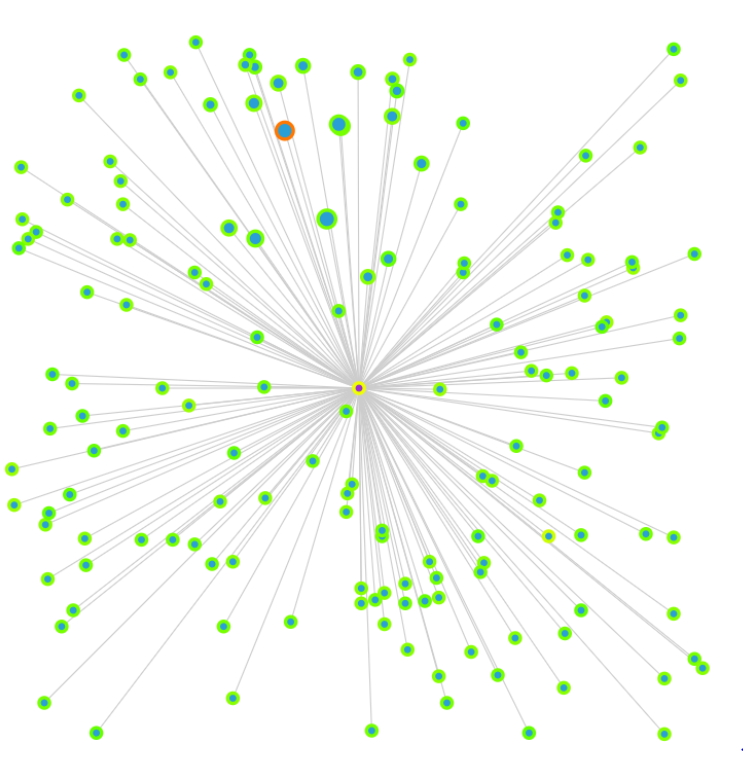
\includegraphics[scale=0.2]{Graphics/nodePresentaion.PNG}}
\caption{Graph Presentation of Nodes in a Network}
\label{fig}
\end{figure}
\vspace{0.5cm}

\section{Theoretical Background} 
\subsection{Internet Topology}

The topology of the Internet forms a clear hierarchy. As we model it in fig. 3, on the lowest level of the Internet topology are Internet Protocol network interfaces (IPs). Multiple IPs can access the Internet through one router (R). Then, on the next level, Autonomous Systems (AS) represent a set of routers under a single administration. For example a large organization like a university consists of multiple intersections with the Internet through its routers. The top of this hierarchy is formed by Internet Service Providers (ISP). As their name suggests, ISPs provide access to the Internet. Note that this represents a simplified and high-level model of Internet topology, i.e. not specifying Points of Presence \cite{ASH}. In the scope of this paper the level of Autonomous Systems is our main object of concern. Two types of relationships between ASes and ISPs are of interest in that regard: Provider-to-Customer (P2C) and Peer-to-Peer (P2P). An Autonomous System, if it functions as a customer in general has only one provider, whereas it usually has many peers. 
 

\begin{figure}[htbp]
\centerline{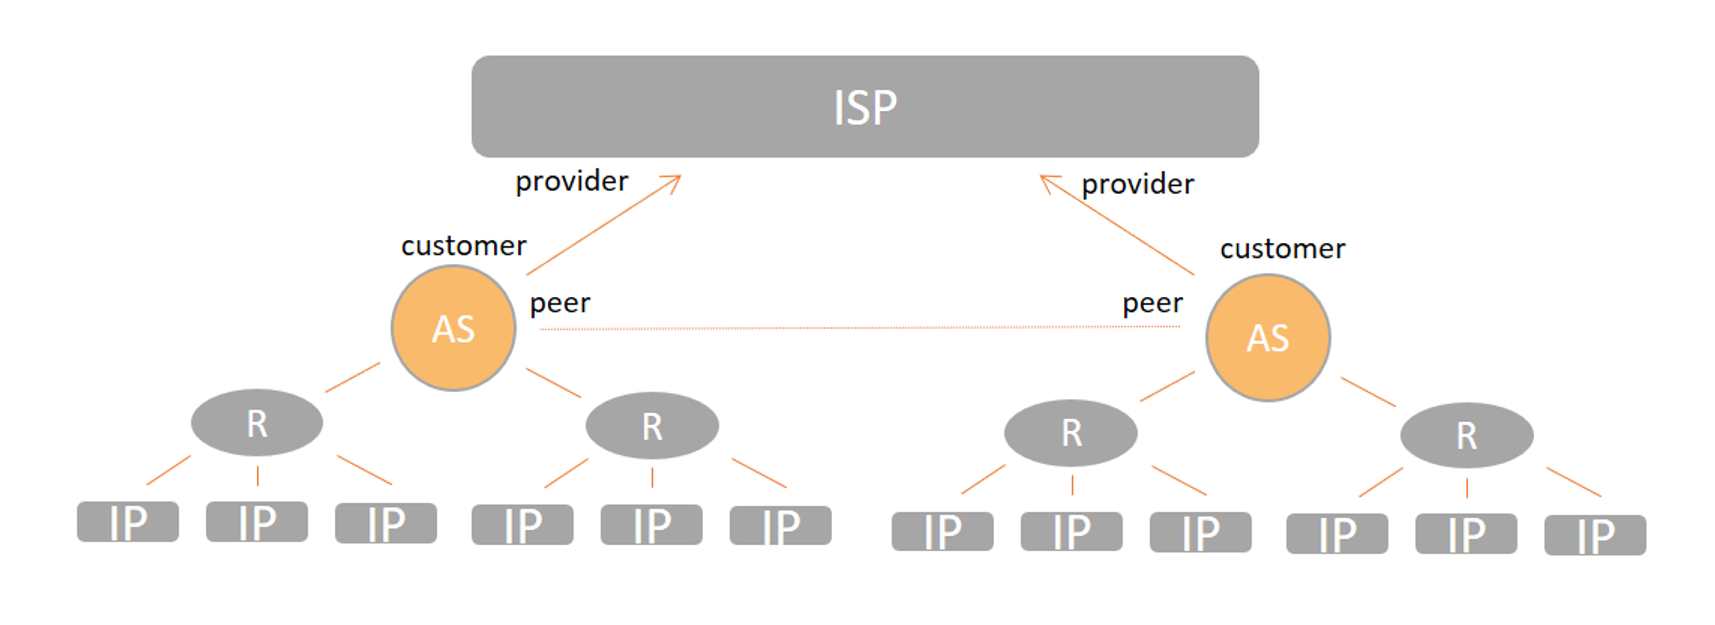
\includegraphics[scale=0.26]{Graphics/hierarchy.PNG}}
\caption{Hierarchy of the Internet}
\label{fig}
\end{figure}
\vspace{0.5cm}





Fig. 4 provides an example of an AS and its characteristics. Here Kabel Deutschland, a German network operator, represents an AS. Its customer cone specifies  ``a set of ASes it can reach using customer links''\cite{Rank}. As it is two in this case, there are only two nodes reached through customer links, meaning Kabel Deutschland itself and its provider Vodafone\cite{Rank}.  
%https://www.caida.org/~amogh/papers/asrank-IMC13.pdf
AS rank defines the importance of a node in its global routing system, often using customer cone information as a measure \cite{Rank}.
%http://as-rank.caida.org/about#goal
\textit{AS degree} refers to the number of neighbors that a node has in a graph on its own level - here 20\cite{Cone}.  \\

\vspace{0.5cm}
\begin{figure}[htbp]
\centerline{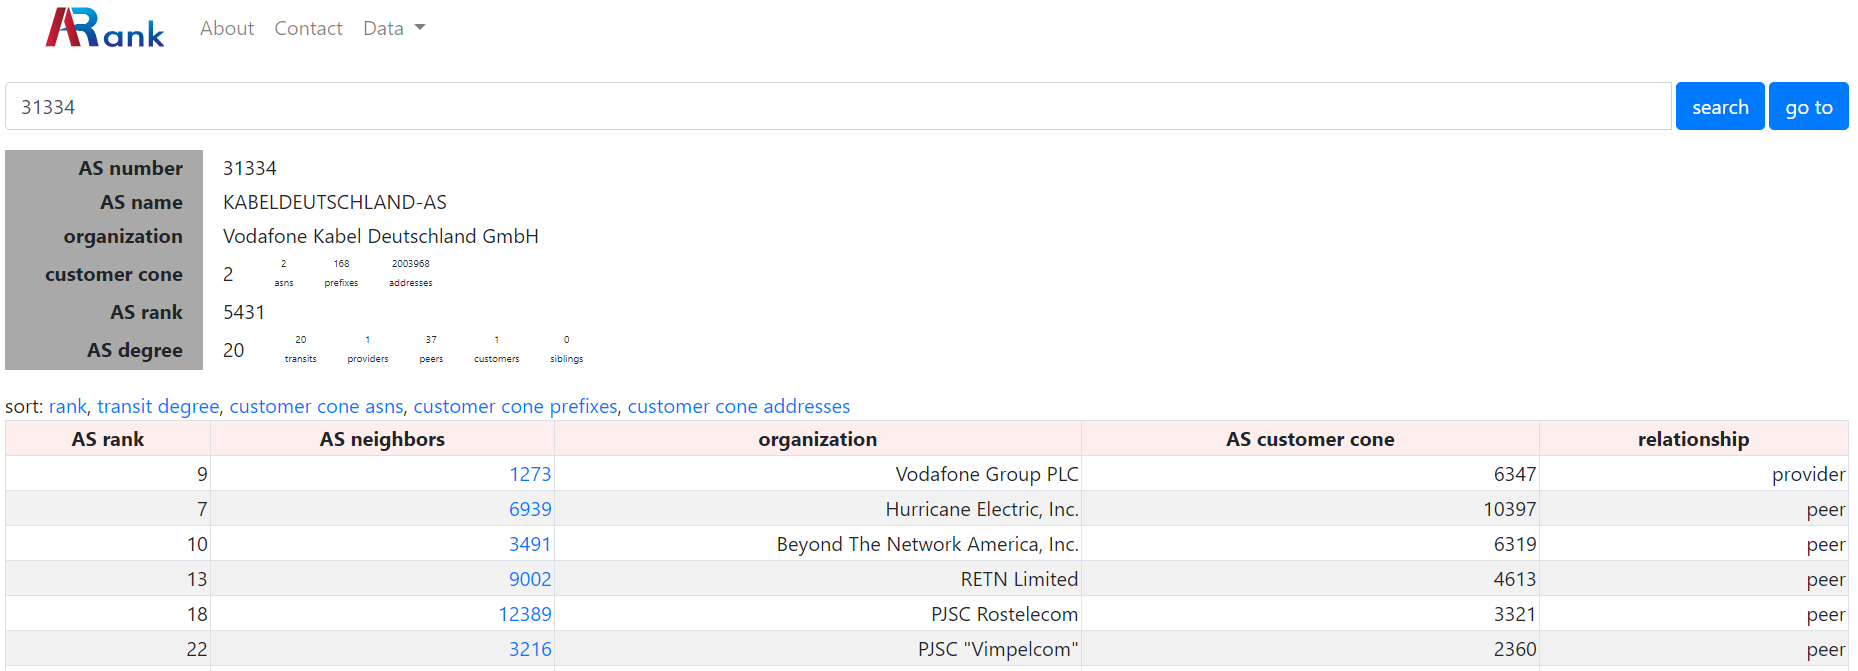
\includegraphics[scale=0.21]{Graphics/asExample.PNG}}
\caption{Example of an AS and its characteristics}
\label{fig}
\end{figure}
\vspace{0.5cm}



\subsection{Internet Robustness}
The Internet is assambled based on the hierarchy as shown in figure 3. Much research has already been conducted on the robustness of the Internet. Baumann and Fabian \cite{howRobust} state the following: While the Internet is resistant with respect to random failures of nodes, a targeted attack such as a degree attack can have a serious impact. The latter stands for an attack that focuses on the successive deletion of nodes with the highest node degree. It was also pointed out that a targeted removal of only ten percent of the nodes of the network can lead to more than 32 000 disjoint components. Further research suggests that due to its evolution the Internet network  is ``robust yet fragile''\cite{RYF}, meaning that random failures of nodes leave the network unaffected, whereas it is vulnerable to targeted attacks on its key components. Acoordingly, the Internet is often reffered to as ``scale-free'' with a ``hub-like'' core structure, which leads to the described characteristics \cite{RYF}. \\ Faloutsos et al. \cite{powerlawCitation} state in their research that the Internet network is following a so called power-law distribution. Power-laws describe skewed distributions of graph properties, such as node degree or betweenness centrality. It can be used for estimating further characteristics of networks or an analysis of robustness. Note though that they base their research on data from November 1997 and December 1998. J. Ruiz and G. Barnett also make statement about the imbalancedness of the Internet \cite{owningInternet}. Their results indicate that the United States is the most central nation in the network, with American corporations accounting for almost 40\% of international links between nodes. Moreover they state that there exists a center of the network consisting of 16 companies, each causing more than 1\% of international Internet connections. Amongst others are the well known companies like Google, Facebook or Amazon. \\ \linebreak
Research of \cite{geoResearch} in 2002 modeled the Internet's large scale topology - amongst others the geographic locations of routers. In that regard, they published the geographic locations of routers and found a major concentration in North America and Europe, which represent western economies that are highly developed in terms of wealth and technological endowments, and less activity on other, less developed continents.\\  \linebreak
 


\subsection{ETL Process}
The data warehousing concept of \textit{Extraction, Transformation, Loading} (ETL) became a rising standard for companies in the 1970s. Back then organizations began to integrate information from different sources into their own databases \cite{carl1}.\break The integration process states the advantage that disparate sources and hereby diverse formation of data can be brought into a unified database. With an adjustable ETL process one is able to adapt and import new datasources without 
changing the essential main system or framework. This segregation of data import and processing makes the whole system more stable, flexible, provides improved maintance and makes it easier for developers to change and extend functionalities. Fig.6 describes this process in general. At the beginning data are extracted from various sources. The extraction must be customized to the characteristics of the respective data provider. These can differ in the file and data format as well as in the interface. For instance, common interfaces are protocols such as \textit{http} or \textit{ftp}, source-specific APIs or stream data.
In the transformation part demanded information are converted into the neccessary database format. As well calculations can be applied, duplicates will be erased, units converted or further algorithms can be applied. 
The last stage is contained in the upload or import into the data warehouse, from where to information can bendrawn from multiple stakeholder . An important requirement in the loading phase states the efficiency: data must be sent within a short duration. Dependent on the size of data, parallelization or hardware adjustments may help in all three sections. (\url{https://link.springer.com/chapter/10.1007/978-3-642-32584-7_6})
\linebreak %Quelle 




\vspace{0.5cm}
\begin{figure}[htbp]
\centerline{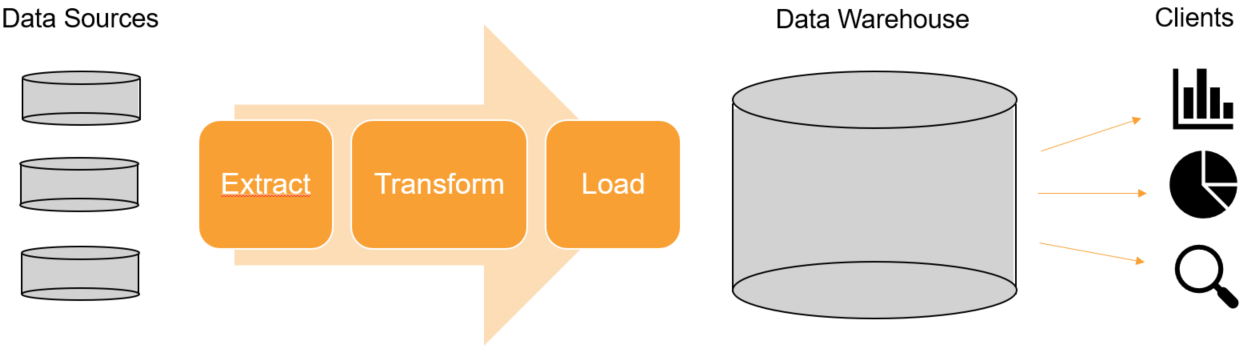
\includegraphics[scale=0.3]{Graphics/ETLTheory.PNG}}
\caption{Theoretical ETL Process}
\label{fig}
\end{figure}
\vspace{0.5cm}



\section{Data}
As a data source for this work, we exclusively focus on Caida. Caida is an abbreviation and stands for Center for Applied Internet Data Analysis. Located in San Diego, CA in the United States, the center studies networks and its infrastructure up to a large scale. For their investigation on theoretical and practical aspects of the Internet they monitor, collect, analyze and provide network data \cite{Caida}. \\  \linebreak

Regarding the data granularity our primary focus lies on AS level data. Within this domain, we investigate five type of datasets. \textit{AS-Rank} offers a data base giving information about specific autonomous systems, like its rank, relationship to other ASes or customer cone  \cite{Rank} . \textit{AS Classification} represents a dataset including information on the business types of Autonomous Systems \cite{Classification}. Through machine-learning inference, Caida is able to offer this knowledge  \cite{Classification}. A large collection of datasets named \textit{Pv4 Routed 24 AS Links} is used in detail to investigate the topology on the Internet, its structure regarding streams of traffic, and ratios of sending and receiving autonomous systems  \cite{IPv4Data}. This collection of data forms the center of our investigation. From 2007 to 2018 data is collected, by three \textit{teams}. Caida uses independent teams to collect data in order to offer a way to validate the data and its data inference. The teams probe every routed /24 in the IPv4 address space.
We investigate the dataset \textit{AS Relationships} in order to find out about Provider-to-Customer relationships as well as Peer-to-Peer relationships \cite{CaidaRelationshipsData}.  Lastly, we take into account geographic information of the Autonomous Systems to draw conlclusions on regions with high imapact on the Internet network and less involved ones  \cite{CaidaGeoData}. For the purpose of investigating the characteristics of ASes itself and their network, we analyzed recent data of December 2017.  As for the time series analysis, we used data from 2007 until 2017. \\


\section{Results}

\subsection{Data Analysis}
First aspect of the data analysis process is the type of autonomous system. Caida distinguished here between three types, as fig. 6 shows as well: The first type are ASes that provide Internet access or function as a transit. They make out 42.2\% of all nodes in the network. Second type are ASes providing content hosting and distribution systems, like Dropbox or Google, with only 4,5\% of all overall nodes. Third category are enterprises meaning organizations, universities or companies that are mostly users. They account for 53.3\%. Insights we are gaining from this aspect is that most of the nodes are representing users of the Internet, which makes intuetively sense. More interesting is the large amount of transits and access points needed to provide the respective infrastructure. This hints to the Internet's high complexity (fig. 7).

\vspace{0.5cm}
\begin{figure}[htbp]
\centerline{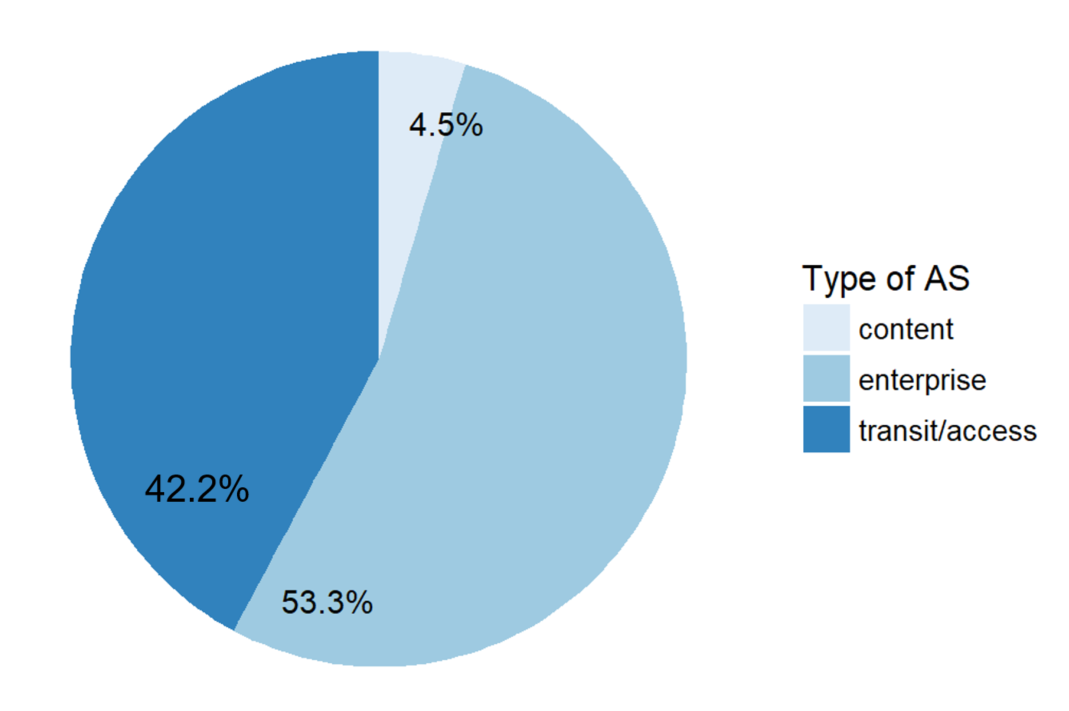
\includegraphics[scale=0.4]{Graphics/typeofAS.PNG}}
\caption{Ratio of Autonomous Systems regarding their Type }
\label{fig}
\end{figure}
\vspace{0.5cm}

As depicted in the theoretical part, autonomous systems have relationships as they transfer data through the web. We took a look at this characteristic in fig. 8 and noticed quite a balanced ratio of Provider-to-Customer relations and Peer-to-Peer relations. If we translate this into a graph, we imagine a balanced graph, which in terms of network riskiness, is rather roboust. 



We furthermore built graphs describing the distributional characteristics of autonomous systems. Fig. 9 shows the distribution of autonomous systems and how many outgoing connections the single nodes have. Approximately 5.500 sending nodes are containted within that data set. We ranked them on the x-axis. With the number of connections an AS is sending to on the y-axis, we obtain a very left centered distribution. A very small number of nodes in the network are sending traffic to a high number of other nodes. It follows, what is called a power-law distribution  \cite{powerlawCitation}.

\vspace{0.5cm}
\begin{figure}[htbp]
\centerline{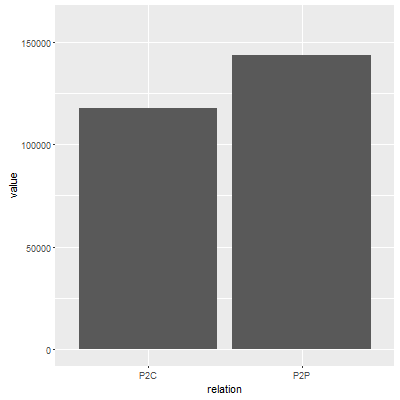
\includegraphics[scale=0.45]{Graphics/relationspeerandprovider.png}}
\caption{Ratio of AS-Relationships }
\label{fig}
\end{figure}
\vspace{0.5cm}

 Calculating the quantiles of the distribution, the top 10 percent of highest ranked nodes (ranked by the number of different outgoing connections) send to almost exactely 50\% of overall trafic of the whole network. The top five percent are responsible for 36\% of all outgoing traffic and the top one percent even accounts for approximately 17\%. \\ \linebreak Note that when we make statements of the whole network, we only refer to the data at hand as the whole network. That is the data collected by Caida. It should also be mentioned that \textit{traffic} in this context is the number of connections and not amount of transferred data. Information on Caida's data collection process can be found in \cite{CaidaDataCollection} . \\ \linebreak

%> sum(sumAsTo$count[1:4900]) / sum(sumAsTo$count)
%[1] 0.5059264
%> sum(sumAsTo$count[1:2450]) / sum(sumAsTo$count)
%[1] 0.3608107
%> sum(sumAsTo$count[1:490]) / sum(sumAsTo$count)
%[1] 0.1678801

Simultaneousely, we drew the distribution of incomming connections per Autonomous System (Appendix A) and received a similar result. With approximately 250.000 nodes, receiving traffic, only very few nodes are receiving traffic from a high number of nodes, again following the properties of a power-law distribution. The top ten percent of highest ranked nodes, are receiving approximately 52\% of the overall traffic in this network. The top five percent make up 36\% and the top one percent even 17\% of overall trafic. The quantiles are almost identical to those of the previous distribution. Such results hint to the Pareto Principle stating that a small number of participants have a large impact on the overall activity and the large majority only accounts for a small influence. This principle has already been proven to be a good estimate for applications in business and economics. Our results suggest that this principle is also feasible for Caida data on AS-level.  \\ 

%top 1 percent
%> sum(sumAsTo$count[1:520]) / sum(sumAsTo$count)
%[1] 0.1724906


%top 5 percent
%2500 / 52055  = 0.05
%> sum(sumAsTo$count[1:2500]) / sum(sumAsTo$count)
%[1] 0.3646528
 

% 10 percent
%> sum(sumAsTo$count[1:5200]) / sum(sumAsTo$count)
%[1] 0.5174527

An important finding regarding connectivity risks of the network is, how vulnerable this network is. An attack targeting the most active and most influential nodes in the network, achieving a non-functioning of those quickly leads to wide shot-downs of the network. Previous introduced results by \cite{powerlawCitation} and \cite{owningInternet} can therefore be supported.  This again underscores the demand for Coria - a tool to analyze connectivity risks for an safe and ongoing network infrastructure 

\vspace{0.5cm}
\begin{figure}[htbp]
\centerline{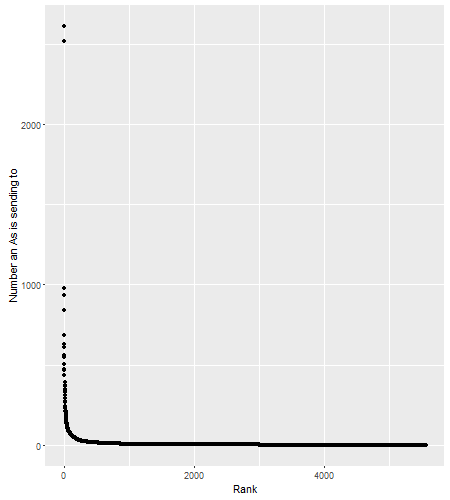
\includegraphics[scale=0.4]{Graphics/AsFromDistribution.png}}
\caption{Distribution of Outgoing Connections per AS}
\label{fig}
\end{figure}
\vspace{0.5cm}


Next, we analyzed the geographic locations of autonomous systems and their flow of traffic. Fig. 9 symbolizes autonomous systems as organge points on a word map. We can see a high concentration of ASes in North America and Europe. The concentration of ASes is less dense in areas like South America, Africa or Asia. Insights that we can draw from that representaion are that more autonomous systems are situated in highly developed economies  than they are in less developed regions. This result corresponds to previous research conducted by \cite{ResearchGeo}. While we need to keep in mind that we are only analyzing one data set - with challenging data collection on top of that, we can assume this result still to be a representative sample of the overall network \cite{CaidaDataCollection}. The results confirm the assumption that most traffic is taking place between parties of richer and more developed economies. Conclusion for these findings may be that the internet is a main driver of any economic growth as well as the leading instrument of communication.

These results confirm the research from 2002 by \cite{geoResearch} and lead to the conclusion that the geographically speaking the Internet network did not develop much further. Accordingly, one can state that developed areas increased their power and wealth, whereas in the last 15 years the development of less wealthy areas is only marginal. Even though we are looking at the level of Autonomous Systems and \cite{geoResearch} looked directly at the router-level, the comparison remains valid. \\


\vspace{0.5cm}
\begin{figure}[htbp]
\centerline{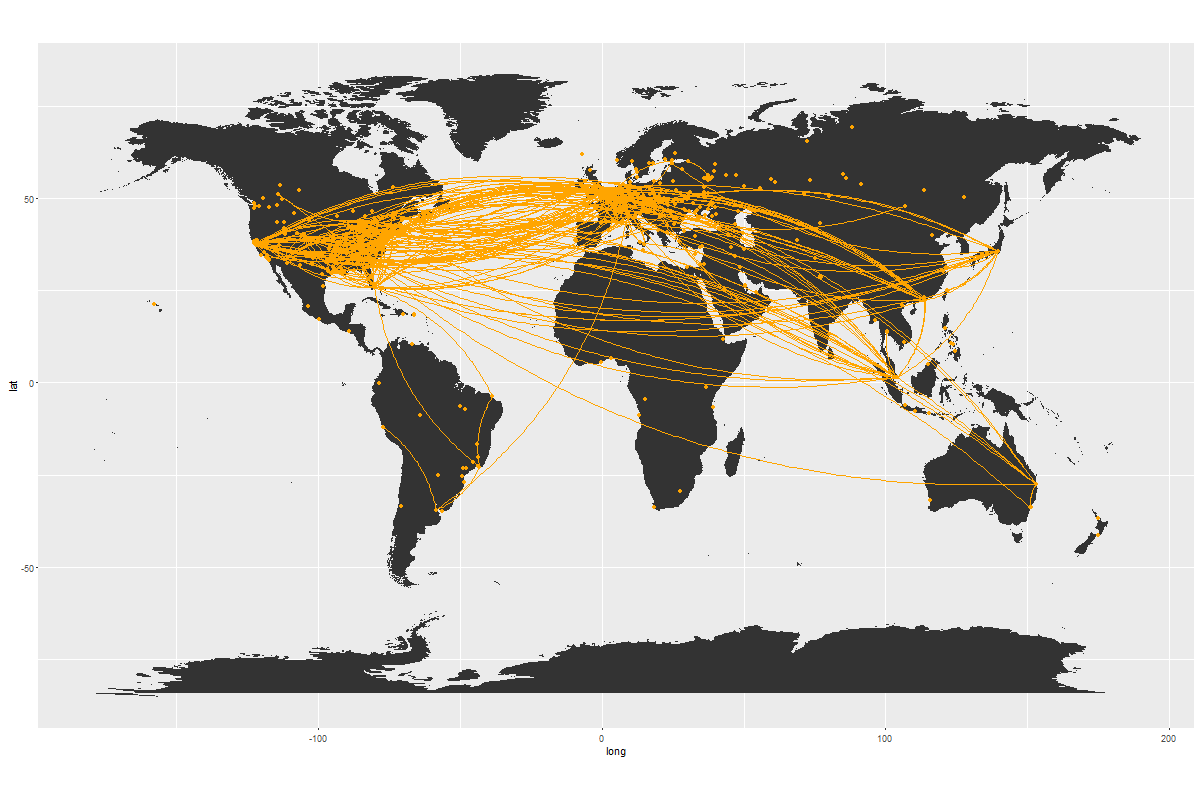
\includegraphics[width=\columnwidth]{Graphics/connectedASes.png}}
\caption{Location of ASes and respective Streams of Traffic}
\label{fig}
\end{figure}
\vspace{0.5cm}

In addition to the analysis of a single point in time, we investigated the timely development of the network. Figure 10 shows the number of traffic-sending autonomous systems from the beginning of 2007 until the end of 2017. Within these 10 years, there is a clear upward trend. In 2015 this upward trend vanishes and and reaches a constant level of approximately 5.500 sending AS nodes within the network. (Note the consistency of results with respect to  the `Distribution of number of sending ASes` in the appendix) Striking in that graph are the multiple outliers appearing throught the time series. A qualitative research about exeptional events happening on these dates that might have been the reason for a downtime of multiple nodes did not lead to reasonable results. As a consequence, we assume the outliers to be caused by monitoring and data collection problems of CAIDA \cite{CaidaDataCollection}. Events like updating the monitoring system can cause such a down time. 

With respect to Appendix .....  you can see a simultaneous development for the amount of nodes, receiving traffic - on a level of approx. 250.000 nodes of course. 

\vspace{0.5cm}
\begin{figure}[htbp]
\centerline{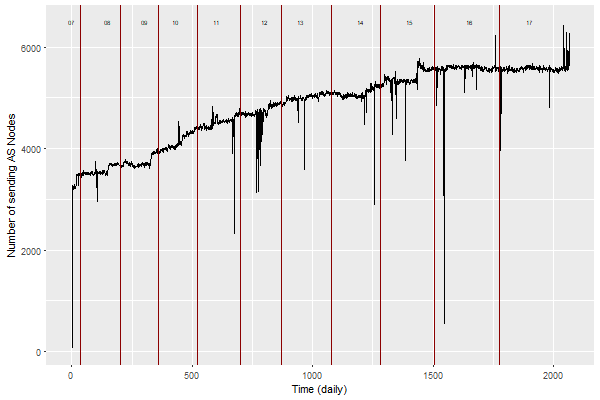
\includegraphics[scale=0.4]{Graphics/ASFromAll.png}}
\caption{Time development from 2007 - 2017: Number of sending AS nodes}
\label{fig}
\end{figure}
\vspace{0.5cm}



\subsection{ETL Process in Coriav3}

This paper is based on the framework of Sebastian Gross\cite{Coria3}. At the current state Coria does not does not provide the functionality of an automated ETL process for any data source. 
The extraction part is handled manually by downloading the desired files and, if neccessary, unzipping the text-formatted file that for instance can be an edge list. \break


The user can now upload the file using the Coria web interface. This can be done through the upload module, following this link: \url{http://141.20.103.31:8080/Coria/#!/datasets/upload}\footnote{If Coria is implemented on an other system the IP changes}. The upload module itself already provides Caida specific upload functions that can handle Caida's file format \cite{Coria3}. Furthermore a "Standard tab seperated Importer" allows users to import edge lists from other data sources. At this time Coria only accepts and deploys solely undirected and unweighted graphs. Users therefore need to be able to adjust or transform their files into the demanded format. The current transformation part in the web framework consists of adjustments that has to be done by the user.\linebreak

\vspace{0.3cm}
\begin{figure}[htbp]
\centerline{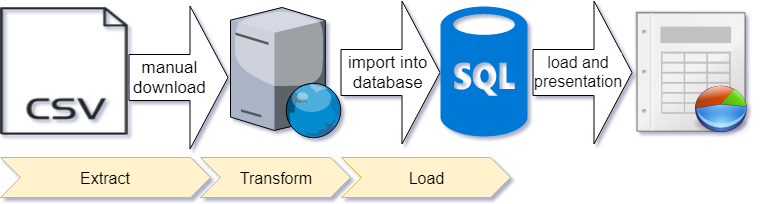
\includegraphics[width=\columnwidth]{Graphics/CoriaETL_current.png}}
\caption{Coriav3: Current ETL Process}
\label{fig:ETLinCoriav3}
\end{figure}
\vspace{0.3cm}



After manually preprocessing the dataset, the web framework allows the user to upload the edge list and then analyze and apply metrics to the data.
Coria already provides an module that can upload data into a MySQL or Redis database. Unexperienced users do not need to be familiar with database management systems. Regarding the upload, loading in the Coria ETL process is already automated. \break
As stated before the performance requirements, uploading files parallel is at the moment not possible. Applying a small penetration test using two clients each uploading two files at the same time, Coria was not able to handle any of the four files. The fact may influence the contributed ETL process as it is running in the background and using the same interface(see: ~\nameref{ssec:contribution}).   \linebreak



\subsection{Contribution: Automated ETL process} \label{ssec:contribution}

Figure \ref{fig:ETLinCoriav3} visualizes the new developed ETL Process, written in Python 2.7. In general, the server periodically queries for new data sets on the Cadia data server. If there are no new data available on the servers the query will try in the next period again. 
In case that there is new data available, every new file will be downloaded. After fetching a new file, it will be transformed into an edge list and then be uploaded to the Coria database.
\linebreak
\linebreak

\vspace{0.5cm}
\begin{figure}[htbp]
\centerline{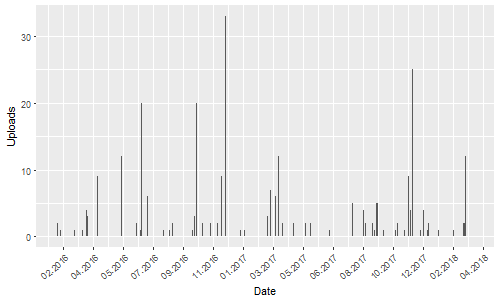
\includegraphics[scale=0.5]{Graphics/uploadFrequency.png}}
\caption{Data Uploads by Caida over time}
\label{fig:UploadOverTime}
\end{figure}
\vspace{0.5cm}


To be more specific, we ensured that the automated ETL process and all of its components trigger every day, we created a function \textit{timer.py} \cite{timer.py}. The timer program is meant to operate permanently and check wether Coria's webservice and the MySQL database are functioning. An 24 hour interval is deemed to be adequate as Caida\textquotesingle s data files provides an snapshot of one day. %carls? was ist das für ein character char13...?

One aspect that we are not in control of, is the frequency and regularity of file uploads by Caida teams. Figure \ref{fig:UploadOverTime} presents a rather unsystematically pattern of uploads. As one can observe in the histogram there are some days with more than 20 uploaded files per day. As well one can also identify periods in summer and around new years eve with none or only a few uploads that can be assumed as holidays. Bearing this in mind, an automated ETL Process can only produce a data input as stable as its data source allows it to do so.
%@DavBer: Was meint der letzte Satz? 
For other sources or data sets the interval can be customized by changing the sleep timer in units of seconds (Listing~\ref{lst:timer}: \lstinline{Frequency = 60 * 60 * 24}).\linebreak


\lstinputlisting[language=Python, caption={timer.py}, label={lst:timer}, firstline=2, captionpos=b,  xleftmargin=.02\textwidth, linewidth = 0.95\columnwidth]{CodeFiles/CoriaETL/timer.py}



The timer program also makes use of \textit{syntax errors and exceptions} \cite{PythonDocumentation}.
From our coding experience with infinite Python loops chances are high for creating unsystematically errors. Amongst others that can be network errors, problems in the operating system on the destination or source server or other faults that can break up the automated ETL process.
Therefore the timer function contains the \textit{continue}-operator in combination with exception handling: If one of the functions creates an error, it can be assured that one day later the ETL porcess will be triggered again without having any person restarting the process or bug fixing. \linebreak

\vspace{0.2cm}
\lstinputlisting[language=Python, caption={main.py}, label={lst:main}, linerange={1-5,8-12},captionpos=b, xleftmargin=.02\textwidth, linewidth = 0.95\columnwidth]{CodeFiles/CoriaETL/main.py}
\vspace{0.5cm}

%@Davber: Kann man in url Bold texten?
The folder structure of Caida's AS Rank files is determined as follows: \textit{\url{http://data.caida.org/datasets/topology/ark/ipv4/as-links/_YEAR_/}}. Therefore the \textit{main} program requests the current year and the year before. The year before has to come into consideration for the case of a new year: Files from December are always uploaded from the teams in the following year. For instance the information from 21 December 2017 was uploaded almost 3 weeks later on 10 January 2018.

Next, at the beginning of the while loop \textit{main.py} creates a connection to data source. As the current year is 2018, the loop starts with calling the webpage of 2017:\textit{...datasets/topology/ark/ipv4/as-links/2017/}. After the connection was established, the module \textit{lxml.html} fetches all links of the website and sets a list out of these.


\lstinputlisting[language=Python, caption={main.py - Link Extraction}, label={lst:main_linkextract}, firstline=17, lastline=27, captionpos=b,  xleftmargin=.02\textwidth, linewidth = 0.95\columnwidth]{CodeFiles/CoriaETL/main.py}


Afterwards a for loop extracts for every link the name of the file. This is due to the fact that the functions \textit{CsvCreate} and \textit{Csv2CoriaDB} need the file name as input parameters. The file names used in the ETL automation and in Caida data source are consistent. The following condition searches in every extracted link for the string "cycle-as". The following if condition checks wether the file was already downloaded. All file that has been processed are stored in the folder \textit{CoriaETL/Data/Original/}. If a file already exists on the Coria server it should already be transformed into an edge list as well as been imported into the MySQL database. For the case that a file does not exist, the \textit{else}-part of the function be executed. First, the data is being downloaded and saved as an unzipped text file. 
Then the main program will call the function that transforms the data into an edge list, which will then be passed to the database. 
The while loop \ref{lst:main_linkextract} will continue until the last file of the current year is processed.
\linebreak


% \vspace{0.5cm}

% \begin{lstlisting}[language=Python, caption={main.py - Filename Extraction},captionpos=b, xleftmargin=.02\textwidth, linewidth = 0.95\columnwidth]
% for j in Liste:
% 	j2= j.rsplit('/')[-1]
% 	j3= j2.split('.gz')[0]

% \end{lstlisting}
% \vspace{0.5cm}



\begin{lstlisting}[ language=Python,caption={main.py - File Processing Part},captionpos=b , float=tp,
  floatplacement=tbp] 

if "cycle-as" in j:
	if os.path.isfile("Data/Original/"+j3):
		print "!!Wurde bereits verarbeitet: " + j3
	else:
		print "## Download und Verarbeitung: " + j3
		response = urllib.urlopen(j)
		compressed_file = io.BytesIO(response.read())
		decompressed_file = gzip.GzipFile(fileobj=compressed_file)
		Filename= "Data/Original/" + j3
		with open(Filename, 'wb') as outfile:
			outfile.write(decompressed_file.read())
			outfile.close()
		#Create a Csv file from download 
		CsvCreate(j3)
		#Upload to Coria databse 
		Csv2CoriaDB(j3)

	YearBefore+=1 

\end{lstlisting}


\textit{CsvCreate} creates an edge list from the original file on the Coria server.
For example, the original ASrank list 'cycle-aslinks.l7.t1.c000027.20070913.txt'(folder: Data/Original/), containing the data description and additional data, will be converted into the pure edge list '20070913.txt(folder: Data/Csv/)' With the Python built-in modules \textit{re — Regular expression operations} %\cite{PythonDocumentation2}
the program extracts the starting and destination nodes of every line beginning with a "D" and adds them to the edge list. These cases are referring to \textit{direct} connections between nodes \cite{IPv4Data}. The edge list will be saved in the format \textit{YYYYMMDD.csv}, i.e. \textit{20180216.csv}
\linebreak

\lstinputlisting[language=Python, caption={CsvCreate.py}, label={lst:csvcreate}, linerange={1-5,8-12},captionpos=b, xleftmargin=.02\textwidth, linewidth = 0.95\columnwidth]{CodeFiles/CoriaETL/CsvCreate.py}


Finally \textit{Csv2CoriaDB} is the last component of the automated data import. The initial idea was to directly work with the MySQL database and import the edge list with the Python SQL module, but the Coria framework inserts not only the data set itself, but it also inserts entries for every edge, node and attribute, as illustrated in figure \ref{fig:SQL_schema}. Thus, we decided to write a script that emulates the process of uploading to the Coria web framework through \textit{Selenium} \cite{selenium}. Selenium is a language-open software framework for testing and automation in web applications.\linebreak

The automated import process makes use of \textit{Chromedriver} as Webdriver API, while other browsers such as Mozilla Firefox or Mac Safari can still be applied. For our specific task Chrome outperformed other browsers. It is important that at the initial installation process of the automated ETL framework Google Chrome has to be installed as well as the Chromedriver path needs to be added to the environent variables.

Exactly like the csv creator the database import takes the file name as input parameter.
Afterwards the webdriver requests the Coria upload page. The Selenium method \textit{find\_element\_by\_xpath} enables the webdriver to fulfill the requested fields.
At first Selnium selects the upload method \textit{tab-separated-importer}, then it sends the name of the imported data set, which is always the date in the format \textit{YYYYMMDD}.
From then on the path of the the file is inserted into the \textit{Select Dataset File} section. 
Finally the script simulates a upload button:  \url{"driver.find_element_by_xpath('//*[@id="import"]/button').click()"}. \\

Webdrivers provide a great variety on options. Therefore we decided to run the chromedriver \textit{--headless} (line 10). This ensures that chrome will not open a window. Instead the chromedriver will run in the background and the upload process will not disturb someone that is working on the server. At the end of every chromedriver session the webdriver must be closed (line 45). If this is not applied the loop will create an great amount of process in the background until the server is overloaded.


\begin{lstlisting}[float=*]
from selenium import webdriver
from selenium.webdriver.common.keys import Keys
from selenium.webdriver.common.by import By
from selenium.webdriver.chrome.options import Options
from selenium.webdriver.support.ui import Select,WebDriverWait
from selenium.webdriver.support import expected_conditions as EC
import time,os

chrome_options = Options()  
chrome_options.add_argument("--headless")  

def Csv2CoriaDB(Filename):
	Filename= Filename.rsplit('.')[-2]
	Filename= Filename.split('.txt')[0]
	#download chromedriver and give Path to chromedriver.exe
	driver = webdriver.Chrome("C:\Python27\Scripts\chromedriver.exe", chrome_options=chrome_options)


	#def CsvUpload:
	driver.get("http://localhost:8080/Coria/#!/datasets/upload")
	driver.implicitly_wait(5)

	#select "tab-separated-importer"
	select = driver.find_element_by_xpath('//*[@id="import.providers"]/option[6]').click()

	#send name
	
	element = driver.find_element_by_xpath('//*[@id="import.name"]')
	element.send_keys(Filename)

	#choose dataset
	path= os.getcwd()
	file = str(path + "/Data\Csv\\" + Filename + ".csv")

	#file = 'C:\caida\Data_Csv\20180101.csv'
	#driver.find_element_by_xpath('//*[@id="file"]'').send_keys(os.getcwd("C:\Users\Carlimero\Downloads\datastructrue.txt")')
	file_input = driver.find_element_by_xpath('//*[@id="file"]')
	file_input.send_keys(file)
	time.sleep(5)

	#submit data
	driver.find_element_by_xpath('//*[@id="import"]/button').click()

	time.sleep(10)
	driver.quit()

	print(Filename + "uploaded to Coria database")
\end{lstlisting}






\vspace{0.5cm}
\begin{figure}[htbp]
\centerline{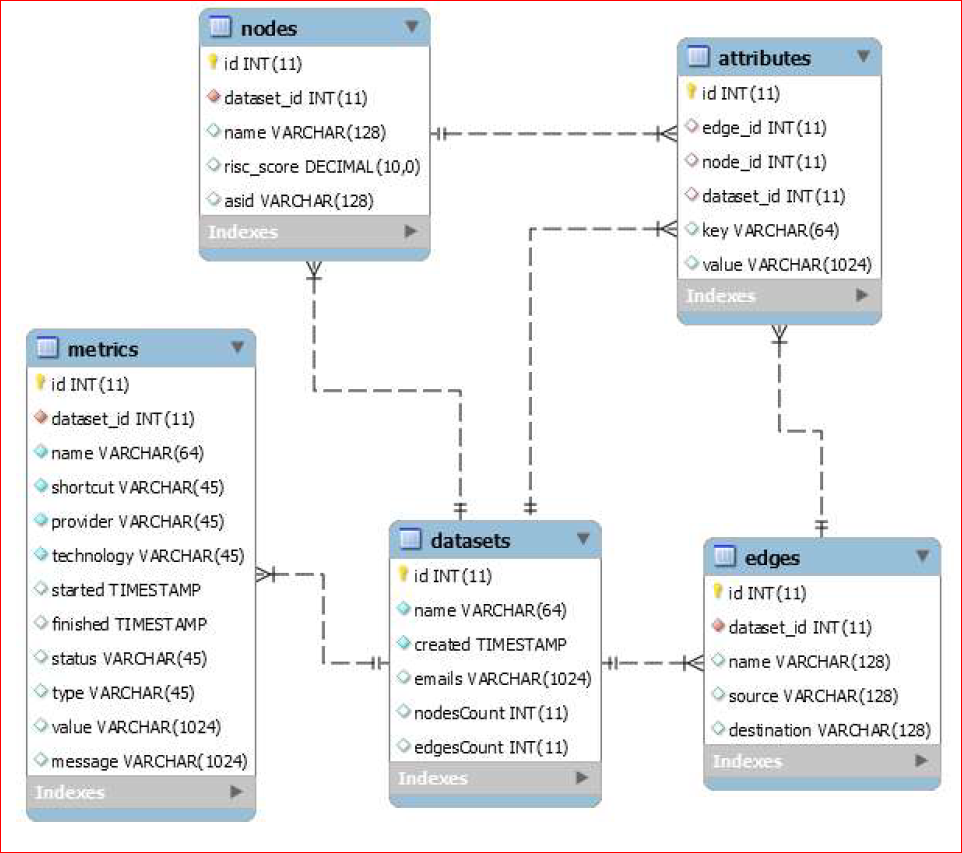
\includegraphics[scale=0.33]{Graphics/SQL_schema.PNG}}
\caption{Relational Database Schema}
\label{fig:SQL_schema}
\end{figure}
\vspace{0.5cm}

\subsection{Initial ETL Implementation}
Caida AS rank data can be tracked back until the year 2007. Garuanteering that a new Coria Server can also work with historic data \textit{InitialDataSetup.py} is provided. Before running the automated ETL process that continuously verifies the presence of newly uploaded data, it is suggested to run the initialisation of the data import once. It should be considered that it takes some hours to compute all historic data. As of today (March 2018), 2160 files have to be processed and imported into the database. We tested the initial data setup, which took a total time of  9:55 hours, testing the script on a virtual server with Windows 2012 R2 with a Common KVM processor 2,53Ghz and 8 GB R.  




\section{Conclusion}
\subsection{Summary}

The webapplication Coria allows the analysis of connectivity risks of various network graphs. Through visualizations and a unified risk score it offers comprehensive results. Fokussing on the level of Autonomous Systems, our data analysis revealed a power-law distribution when it comes to the influence of ASes within the Internet network - a few highly important nodes and many less important ones. Moreover the geographical investigation of its locations showed the high concentration and flow of traffic of ASes in highly developed economies, with only sparse density in less developed economies. With regard to the trend of the Internet network, we exhibited a linearly growing trend of AS nodes until 2015, when the size of the network stayed constant until today.

Regarding the software-development aspect, we developed an ETL tool in Python 2.7 that provides modules for an automated ETL process. Hereby we developed components that are capable of checking for new data, downloading it and providing validation functionalities - without any manual interference. Moreover these files then are being imported into the Coria framework, which enables the possibility of using the lattest data for the analysis of connectivity risks. \\
 

\subsection{Limitations and Further Work}
One limitation of this work is caused by our data source Caida. The data that we used, i.e. types of Autonomous Systems or their relationship was partly gathered through statistical inference. Its machine learning classifier provided a positive predicted value of 70\% \cite{Classification}, which still leaves misslassified observations within the data and limits our results to some extent. Nevertheless Caida is a serious and trusted source, which is why we chose it in the first place. To the best of our knowledge, there is no superior data source available.  \\ 

other limitations\\ 
carl? \\



Further work that can follow could be to apply the automated ETL process to further data sources, than only Caida. Also, deploying the the Coria framework on a server would be a neccessary improvement. (CARL? Was hat es mit diesem Punkt auf sich? Läuft es nicht schon auf einem Server?) For improvements of internal development activities the creation of an extensive code and installation documentation would be helpful.



\begin{thebibliography}{00}
\bibitem{dyn}K. York. (2016, Oct.) Dyn’s Statement on the 10/21/2016 DNS DDoS Attack, [Online]. Available: https://dyn.com/blog/dyn-statement-on-10212016-ddos-attack/

\bibitem{DT}E.Auchard. (2016, Nov.)Deutsche Telekom attack part of global campaign on routers, [Online]. Available: https://www.reuters.com/article/us-deutsche-telekom-outages/deutsche-telekom-attack-part-of-global-campaign-on-routers-idUSKBN13O0X4

\bibitem{Ponemon}Ponemon Institute LLC, ``Cost of Data Center Outages,'' Data Center Performance Benchmark Series, 2016 %https://www.vertivco.com/globalassets/documents/reports/2016-cost-of-data-center-outages-11-11_51190_1.pdf

\bibitem{cyberSponsors} By EWEN MACASKILL and GABRIEL DANCE Produced by FEILDING CAGE and GREG CHEN Published on November 1, 2013. Available: https://www.theguardian.com/world/interactive/2013/nov/01/snowden-nsa-files-surveillance-revelations-decoded.

\bibitem{cyberSponsors2}R.Barton, ``Chinese cyberattack hits Canada's National Research Council,'' CBC News. Available: http://www.cbc.ca/news/politics/chinese-cyberattack-hits-canada-s-national-research-council-1.2721241

\bibitem{cyberSponsors3}A.Kharpal, ``North Korea government-backed hackers are trying to steal cryptocurrency from South Korean users,'' CNBC, Available: https://www.cnbc.com/2018/01/17/north-korea-hackers-linked-to-cryptocurrency-cyberattack-on-south-korea.html

\bibitem{Coria}B. Fabian et al., `` Coria – Analyzing Internet Connectivity Risks Using Network Graphs,'' IEEE International Conference on Communications Paris (IEEE ICC 2017), May 2017. 10.1109/ICC.2017.7996828. 

\bibitem{Ehlert}M. C. Ehlert, "A Software Framework for Analyzing Connectivity Risk of Graph Data," Master of Science, Humboldt-Universität zu Berlin, 2014. 

%\bibitem{Coria1} fehlt noch


\bibitem{Coria2} D.Kiene-Maksimovic, E. Zinovyeva, J. Park, ``Coria 2.0: Augmenting a Universal Framework for Connectivity Risk Analysis,'' Jahr???

\bibitem{Coria3}S.Gross, ``Entwicklung eines modularen Frameworks für die Analyse von Verbindungsrisiken von Netzwerken basierend auf Netzwerkgraphen,'' November 2017.

\bibitem{CoriaPaper}

\bibitem{ASH}

\bibitem{Rank}Caida., ``AS Rank,'' [Online]. Available: http://as-rank.caida.org/.

\bibitem{Cone}M. Luckie et al., "AS Relationships, Customer Cones, and Validation", Internet Measurement Conference (IMC), Oct 2013, pp. 243--256.

\bibitem{howRobust}Baumann, A., Fabian, B. 2015. “How Robust is the Internet? – Insights
from Graph Analysis,” in Proceedings of the 9th International
Conference on Risks and Security of Internet and Systems (CRiSIS
2014), Trento, Italy, Springer, LNCS 8924, pp. 247-254.

\bibitem{RYF}Albert, R. Jeong, H. and Barabasi, A.-L. (2000) Nature 406, 378–382.

\bibitem{powerlawCitation}M. Faloutsos, P. Faloutsos, and C. Faloutsos, “On power-law relationships of the Internet topology,” Proc. of ACM SIGCOMM ’99, Cambridge, MA, Aug. 1999, pp. 251–262.

\bibitem{owningInternet}J. Ruiz, G. Barnett, ``Who owns the international Internet networks?,'' The Journal of International
Communication. November 2014. 21:1, 38-57, DOI:
10.1080/13216597.2014.976583

\bibitem{geoResearch}S. Yook, H. Jeong, A. Barabasi, ``Modeling the Internet's Large-Scale Topology, '' Proceedings of the National Academy of Sciences of the 
United States of America, November 2002.

\bibitem{carl1}SAS Institute GmbH (n.d.). Retrieved from \url{https://www.sas.com/en_us/insights/data-management/what-is-etl.html}

\bibitem{Caida}Caida, [Online] Available: https://www.caida.org/home.

\bibitem{Classification}Caida., ``AS Classification,'' [Online]. Available: http://www.caida.org/data/as-
classification.

\bibitem{PythonDocumentation}Python Software Foundation., ''6. Built-in Exceptions,'' [Online]. Available: http://www.python.org/2.7/library/exceptions.html.

% \bibitem{PythonDocumentation2}Python Software Foundation., ''7.2. re - Regular expression operations'' [Online]. Available: https://docs.python.org/2/library/re.html#regular-expression-syntax.

\bibitem{IPv4Data}Caida., ``IPv4 Routed /24 AS Links Dataset,'' [Online]. Available: http://www.caida.org/data/active/ipv4\_routed\_topology\_aslinks\_dataset.xml.

\bibitem{CaidaRelationshipsData}Caida., ``AS Relationships,'' [Online]. Available:http://www.caida.org/data/as-relationships/.

\bibitem{CaidaGeoData}Caida., ``AS Relationships -- with geographic annotations,'' [Online]. Available: http://www.caida.org/data/as-relationships-geo/.

\bibitem{CaidaDataCollection} 

%aus unserer Präsi:
%B. Fabian, G. Tilch, “Analyzing the Global-Scale Internet Graph at Different Topology Levels: Data Collection and Integration“.
%D. Kiene-Maksimivic, E. Zinovyeva, J. Park, “Coria 2.0: Augmenting a Universal Framework for Connectivity Risk Analysis”, 2017.
%J. Dümig, “Modelling of an Extraction Transformation Loading (ETL) system for the connectivity risk analyzing framework Coria“, 2016.
%M. Luckie et al., “AS Relationships, Customer Cones, and Validation”, Internet Measurement Conference, 2013.
%M. Oehlers, B. Fabian, ”Graph Metrics for Internet Robustness: A Survey”, ACM Comput. Surv. 1, 1, Article 1, 2018.
%S.Gross, “Development of a modular software framework for the analysis of network connectivity risks based on network graphs”, 2017.
%T. Kober, “Business Intelligence in der Telekommunikation : Konzeption und Umsetzung einer Graphendatenbank mittels Neo4j“, 2016.
%ende aus unserer präsi

\bibitem{powerLaw} Yaneer Bar-Yam. ``Concepts: Power Law," New England Complex Systems Institute, August 2015.

\bibitem{CaidaRelationships}X. Dimitropoulos, G. Riley, ``Modeling Autonomous System Relationships,'' Principles of Advanced and Distributed Simulation (PADS), May 2006, pp. 143--149.

\bibitem{RelInference}X. Dimitropoulos et al., ``Revealing the Autonomous System Taxonomy: The Machine Learning Approach," Passive and Active Network Measurement Workshop (PAM), Mar 2006.

\bibitem{CaidaRel2}X. Dimitropoulos et al., "Classifying the Types of Autonomous Systems in the Internet", SIGCOMM, Aug 2005.

\bibitem{ResearchGeo}

\bibitem{graphMetrics}M. Oehlers, B. Fabian, ``Graph Metrics for Internet Robustness: A Survey,'' ACM Comput. Surv. 1,1, Article 1, January 2018.

\bibitem{BAETL}J.Dümig, ``Modelling of an Extraction Transformation Loading (ETL) system for the connectivity risk analyzing framework Coria, December 2016.

\bibitem{BA}T.Kober, ``Business Intelligence in der Telekommunikation: Konzeption und Umsetzung einer Graphendatenbank mittels Neo4j,'' December 2016.

\bibitem{carl2}butunclebob(n.d.). Retrived from \url{http://butunclebob.com/ArticleS.UncleBob.PrinciplesOfOod}


\bibitem{selenium}SeleniumHQ, [Online] Available: https://github.com/SeleniumHQ/selenium.


%\bibitem{carl3} S. Gross "Development of a modular software framework for the analysis of network
%connectivity risks based on network graphs" (Bachelor thesis), 2017

%mehr Quellen von Prof Fabian:
\bibitem{geoVul}A. Baumann, B. Fabian. ``Towards Measuring the Geographic and Political Resilience of the Internet,'' International Journal of Networking and Virtual Organisations, 13(4):365–384, 2013.

\bibitem{timer.py}

%Damien Magoni. Tearing Down the Internet. IEEE Journal of Selected Areas in Communications, 21(6):949–960, September 2006.

%Martin Huth and Benjamin Fabian. Inferring Business Relationships in the Internet Backbone. International Journal of Networking and Virtual Organisations, 16(4), 2016.

%Annika Baumann and Benjamin Fabian. Who Runs the Internet? Classifying Autonomous Systems into Industries. In Proceedings of the 10th International Conference on Web Information Systems and Technologies (WEBIST), Barcelona, Spain, 2014.

%Annika Baumann and Benjamin Fabian. Vulnerability Against Internet Disruptions – A Graph-based Perspective. In Proceedings of the 10th International Conference on Critical Information Infrastructures Security (CRITIS 2015), Berlin, Germany, LNCS, Vol. 9578, Springer, 2015.

%Benjamin Fabian, Annika Baumann, and Jessica Lackner. Topological Analysis of Cloud Service Connectivity. Computers & Industrial Engineering, 88:151–165, 2015






abstand\\
%die quellen sind nur als Formatvorlage gedacht:
%\bibitem{b1}still old!noch die aus der Präsi einfügen'! G. Eason, B. Noble, and I. N. Sneddon, ``On certain integrals of Lipschitz-Hankel type involving products of Bessel functions,'' Phil. Trans. Roy. Soc. London, vol. A247, pp. 529--551, April 1955.
%\bibitem{b2} J. Clerk Maxwell, A Treatise on Electricity and Magnetism, 3rd ed., vol. 2. Oxford: Clarendon, 1892, pp.68--73.
%\bibitem{b3} I. S. Jacobs and C. P. Bean, ``Fine particles, thin films and exchange anisotropy,'' in Magnetism, vol. III, G. T. Rado and H. Suhl, Eds. New York: Academic, 1963, pp. 271--350.
%\bibitem{b4} K. Elissa, ``Title of paper if known,'' unpublished.
%\bibitem{b5} R. Nicole, ``Title of paper with only first word capitalized,'' J. Name Stand. Abbrev., in press.
%\bibitem{b6} Y. Yorozu, M. Hirano, K. Oka, and Y. Tagawa, ``Electron spectroscopy studies on magneto-optical media and plastic substrate interface,'' IEEE Transl. J. Magn. Japan, vol. 2, pp. 740--741, August 1987 [Digests 9th Annual Conf. Magnetics Japan, p. 301, 1982].
%\bibitem{b7} M. Young, The Technical Writer's Handbook. Mill Valley, CA: University Science, 1989.
%Barabasi, A., Albert, R.: Emergence of Scaling in Random Networks. Science 286(5439) (1999) 509{512
\end{thebibliography}
\pagebreak


\begin{appendices}


\section{Distribution of Incoming Connections per AS}

\begin{figure}[htbp]
\centerline{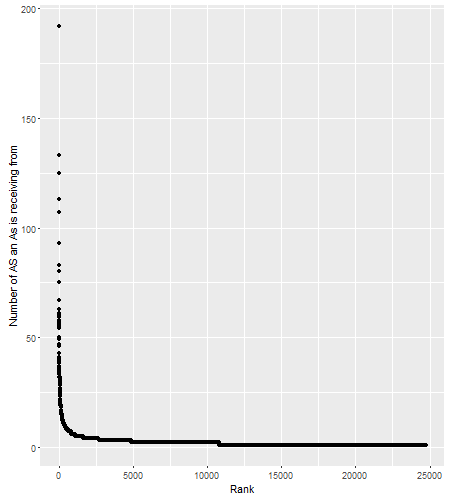
\includegraphics[scale=0.4]{Graphics/AsToDistribution.png}}
\caption{Distribution of Incoming Connections per AS}
\label{fig}
\end{figure}



\section{Geographical Locations of ASes}

\begin{figure}[htbp]
\centerline{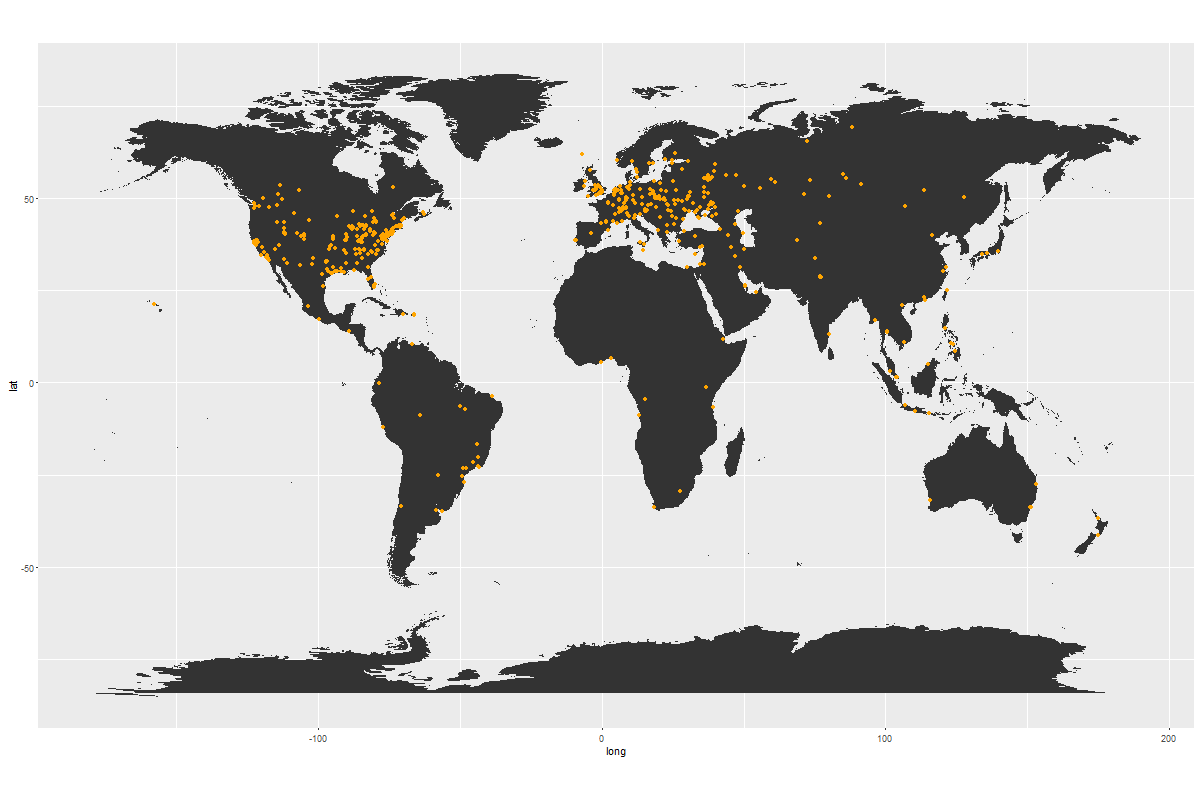
\includegraphics[scale=0.2]{Graphics/ASesNurPunkte.png}}
\caption{Geographical Locations of ASes}
\label{fig}
\end{figure}



\section{Time development from 2007 - 2017: Number of receiving AS nodes}

\begin{figure}[htbp]
\centerline{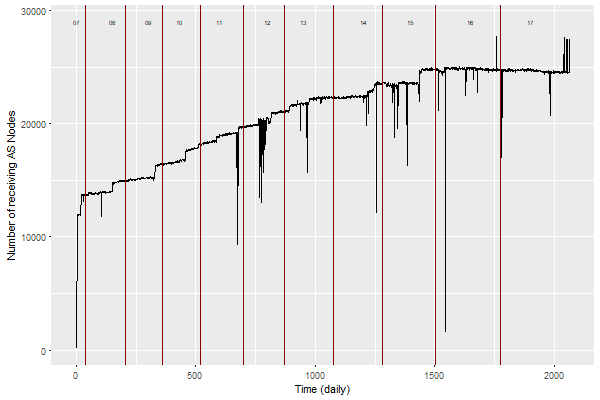
\includegraphics[scale=0.4]{Graphics/ASToAll.png}}
\caption{Time development from 2007 - 2017: Number of receiving AS nodes}
\label{fig}
\end{figure}
\end{appendices}

\end{document}
